\chapter{Timing en optimalizatie}
\label{timing-optimization}
Voor een correcte werking van het geheugen, is het van belang dat de verschillende controlesignalen in een welbepaalde volgorde verwerkt en doorgegeven worden.
Door al de signalen even snel te maken als het kritisch pad is er ruimte voor optimalisatie. In het eerste deel van dit hoofdstuk zal de invloed van architectuur en sizing onderzocht worden op de timing van de signalen. De constraints en vrijheidsgraden die hieruit volgen zullen dan gebruikt worden in het tweede deel van dit hoofdstuk om een optimale architectuur te bepalen.

\section{Timing}
\label{timing}
Het ontwerp van het geheugen in dit werk gaat tot het niveau van het global block (GB) \ref{globalblock}, hierbij wordt de veronderstelling gemaakt dat alle signalen tegelijkertijd binnen komen in het GB. Hierna propageren de signalen door logische poorten tot ze verschillende transistoren rond de BL aansturen. De aansturing van deze transistoren leidt tot de eerste kritische timing constraints. Vervolgens worden de passgates en SA aangesloten, deze zullen de tweede timing constraints bevatten.

\subsection{Kritische timing voor het (de)selecteren cell}
\label{optimization}
\paragraph{}
Timingproblemen die het gevolg zijn van het (de)selecteren van de cel ontstaan door een verschil in timing voor (de)selecteren van de lastimpedantie en cel. Indien de load geactiveerd wordt voor de cel geactiveerd is, zal de bitline vroegtijdig beginnen opladen naar de voedingsspanning. Wanneer de cel dan geselecteerd is zal de bitline naar een spanning getrokken worden die overeen komt met de referentiespanning of een spanning van een cel in RHS of LRS. Afhankelijk van het tijdsverschill tussen deze twee gebeurtenissen, zal de bitline terug omlaag getrokken worden, wat resulteert in een energieverspilling. Dit wordt geïllustreerd in figuur \ref{fig:critisch_timing1}. Indien de cel gedeselecteerd wordt voordat de load gedeselecteerd is, zal de bitline ook opladen naar de voedingsspanning. Dit heeft als gevolg dat het ontladen van de bitlijn langer zal duren of het risico op een leesverstoring vergroot zal worden. Het overbodig opladen resulteert eveneens in een energieverspilling. De passgate die aan de BL hangt, wordt aangestuurd door de controlelogica. Door de opbouw van deze logica, heeft de uitgangsknoop achter de passgate één inverterdelay tijd om te ontladen. Vaak is dit niet voldoende, en zal de uitgangsknoop van het LB niet volledig ontladen zijn. Dit wordt geïllustreerd in figuur \ref{fig:critisch_timing2}.   Dit heeft geen nadelige gevolgen omdat de capaciteit op dit knooppunt heel klein is en er bijgevolg een verwaarloosbare ladingsherverdeling is in de volgende leescyclus. 


\begin{figure}[ht]
\centering
\subfloat[Overshoot van BL omdat load geactiveerd wordt\newline voor WL geactiveerd is]{ 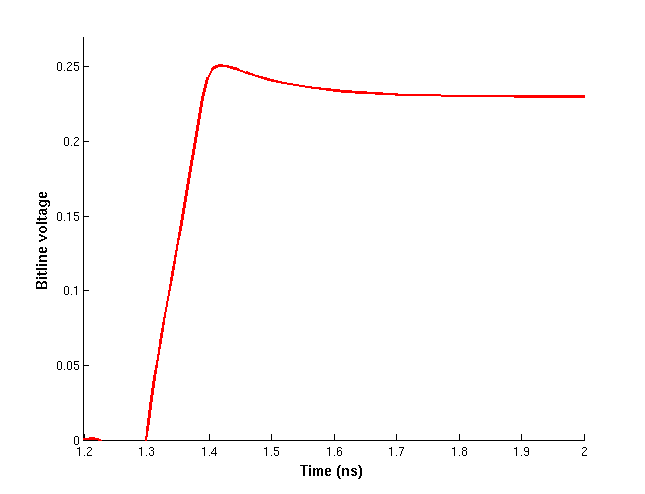
\includegraphics[width=0.55\textwidth] {../fig/hfdstk-timing-crit1.png} \label{fig:critisch_timing1}}
\subfloat[Overshoot van BL omdat load degeactiveerd wordt nadat WL degeactiveerd is]{ 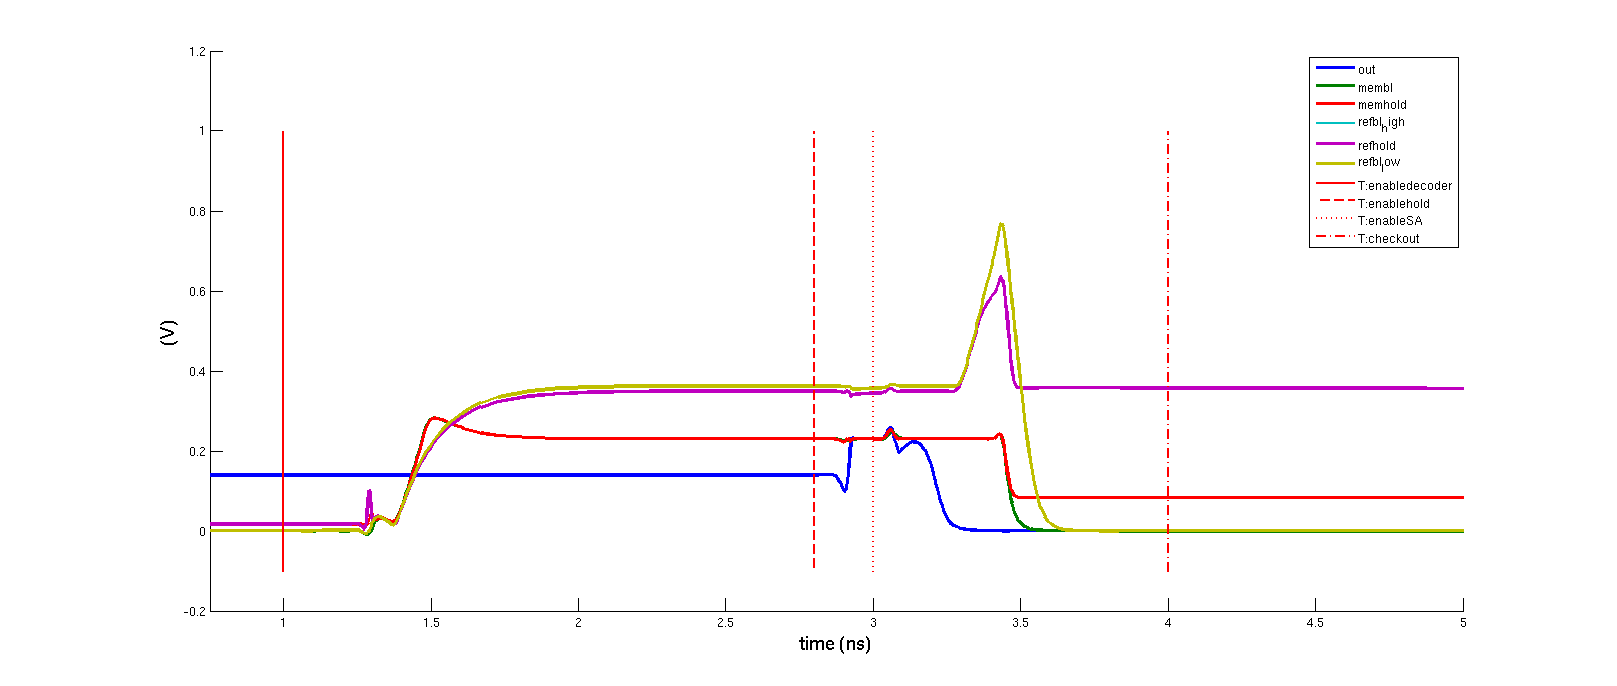
\includegraphics[width=0.40\textwidth] {../fig/hfdstk-timing-crit2.png} \label{fig:critisch_timing2}}
\caption[Timingproblemen bij de bitline]{Timingproblemen bij de bitline}
\clearpage
\end{figure}

\paragraph{}
Er wordt verondersteld dat alle adressignalen tegelijkertijd in het GB aankomen. De timinganalyse start dan ook vanaf dit tijdstip. Het circuit- en timingsdiagram van de logica in het GB worden geïllustreerd in figuren \ref{fig:gb_timing1} en \ref{fig:gb_timing2}. T1 en T2 stellen de momenten voor dat de signalen uit de BL- en WL-decoder komen. T3 stelt het moment voor dat het signaal uit de referentiebuffer komt. T1 en T3 zouden op het zelfde moment moeten aankomen om een optimale timing te hebben. Indien dit niet het geval is, zullen de referentie-BL al geactiveerd zijn voordat de data-BL opgeladen wordt. Indien er een groot aantal referentiebitlijnen zijn, zal dit resulteren in een grote energieverspilling. Er zijn twee opties om de correcte volgorde tussen T1,T2 en T3 te garanderen. De eerste is het kiezen van een kleine BL-decoder en een grote WL-decoder. Dit zal voor een kleine T1 zorgen door een kleine delay in de bitlijndecoder. Dit zal tevens een grotere T3 geven omdat de referentiebuffer een grotere last heeft om op te laden. Een evenwicht kan zo gevonden worden om T1 en T3 op het zelfde moment te doen verschijnen. Deze eerste optie beperkt de mogelijke architectuur aanzienlijk en zal het verwezenlijken van andere timingconstraints voor T2 onmogelijk maken, zoals later zal blijken.\\ 
De tweede optie voor het matchen van T1 en T3 is het uitstellen van T3. Dit uitstel kan gerealiseerd worden door het invoeren van delayelementen of door de buffer suboptimaal te ontwerpen. Het invoeren van delay(vertragings)elementen zorgt in de praktijk echter meestal voor een te grote bijkomende delay. Daarom werd er in het finale ontwerp een buffer ontworpen die niet optimaal is wat snelheid betreft. Om het energieverbruik van de referentiebitlijnen verder in te perken werden niet al de bitlijnen in de array gebruikt voor het genereren van het referentiesignaal.

\begin{figure}[!ht]
  \centering
  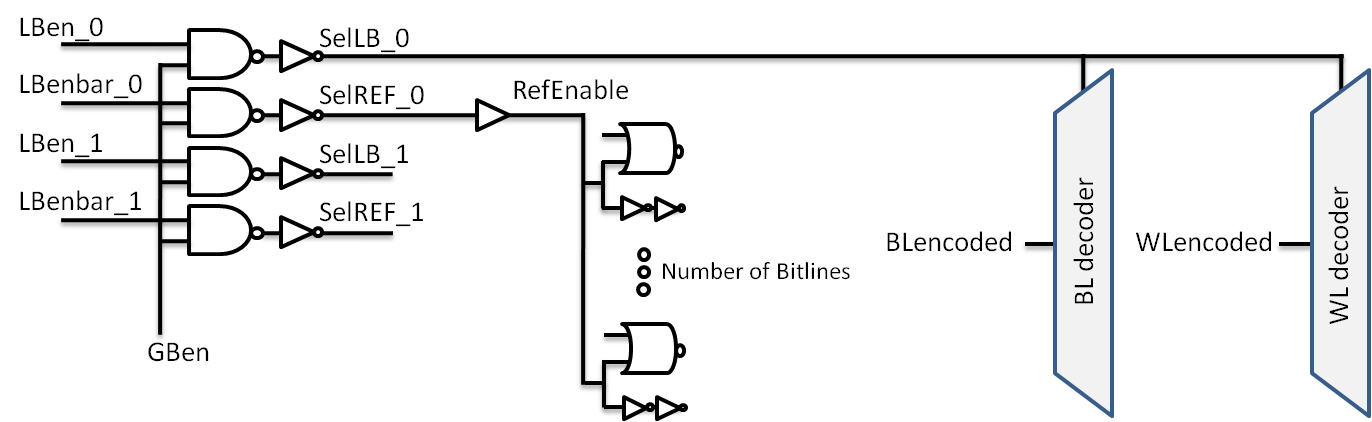
\includegraphics[scale=0.6]{../fig/hfdstk-timing-gb1.png}
  \caption[Global block:logica]{Global block logica}
  \label{fig:gb_timing1}
\end{figure}

\begin{figure}[!ht]
  \centering
  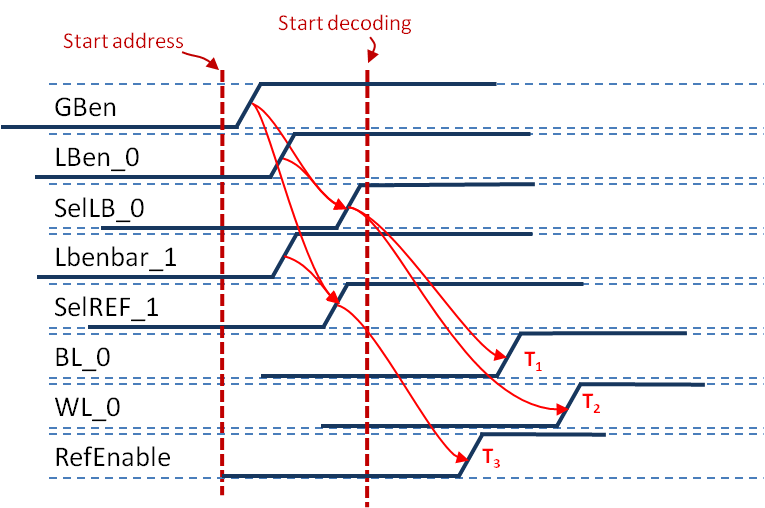
\includegraphics[scale=0.9]{../fig/hfdstk-timing-gb2.png}
  \caption[Global block:timing]{Timing global block}
  \label{fig:gb_timing2}
\end{figure}

\paragraph{}
Eens de sigalen uit de decoders komen worden deze gestuurd naar de controlelogica voor de memory array. Het circuit- en timingdiagram hiervan staan geïllustreerd in figuren \ref{fig:lbcell_timing1} en \ref{fig:lbcell_timing2}. De cel zou vroeger dan of gelijk met de last moeten aangeschakeld worden. Op het timingdiagram wordt dit geïllustreerd als T4 = T5 = T6. Door de implementatie van de logica is dit niet mogelijk aangezien er altijd een inverterdelay verschil is tussen T4 en T5. Deze vertraging is minimaal en kan getolereerd worden omdat de bitlijn in elk geval moet opgeladen worden tot minimum $V_{LRS}$. Bij lage voedingsspanningen wordt dit probleem echter meer uitgesproken. T6 wordt bepaald door WL-decoder en -buffers. Deze vertraging zou zodanig ontworpen moeten worden dat deze vroeger dan of gelijk met T5 valt. Bij het afschakelijken van de cel zijn de omgekeerde voorwaarden nodig. De last zou namelijk vroeger dan of gelijk met de cel moeten afgeschakeld worden. Deze voorwaarde is voldaan als T7 voor T8 en T9 komt. Door de inverter is T7 altijd voor T8. T9 daarentegen wordt bepaald door de WL-decoder en -buffer en zou voor T7 moeten komen. \\
Zoals uit figuur \ref{fig:lbcell_timing1} blijkt, zijn de meeste controlesignalen om een datacel uit te lezen niet onafhankelijk, enkel de timing van het WL-signaal kan vrij aangepast worden. Deze moet geselecteerd worden vooraleer de sourceline geselecteerd is en mag pas gedeselecteerd worden nadat de last gedeselecteerd is. \\
De timing van de wordline wordt expliciet bepaald door de grootte van de WL-decoder en impliciet door de grootte van de BL-decoder. De BL-decoder bepaalt namelijk de delay van de WL-buffer. Figure \ref{fig:decoder_dep} geeft de delay van verschillende groottes van WL-decoders en -buffers i.f.v. verschillende groottes van BL-decoders weer.

\begin{figure}[!ht]
  \centering
  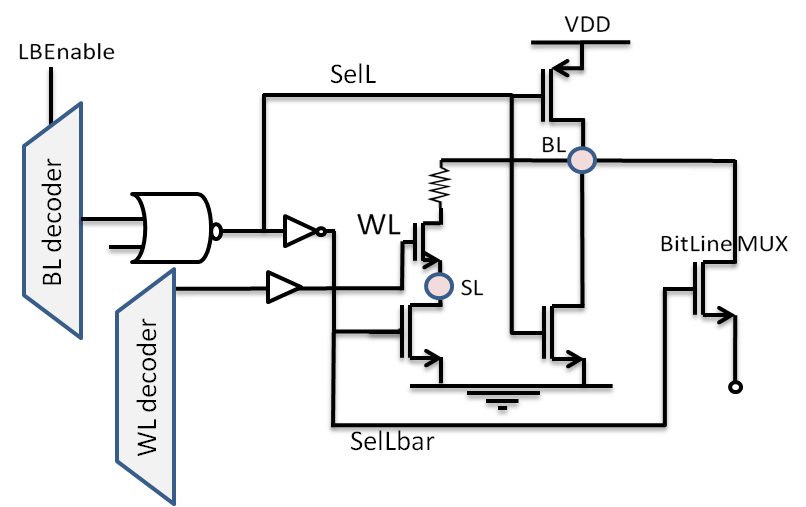
\includegraphics[scale=0.6]{../fig/hfdstk-timing-lbcell1.png}
  \caption[Data-array:logica]{Controlelogica data-array}
  \label{fig:lbcell_timing1}
\end{figure}

\begin{figure}[!ht]
  \centering
  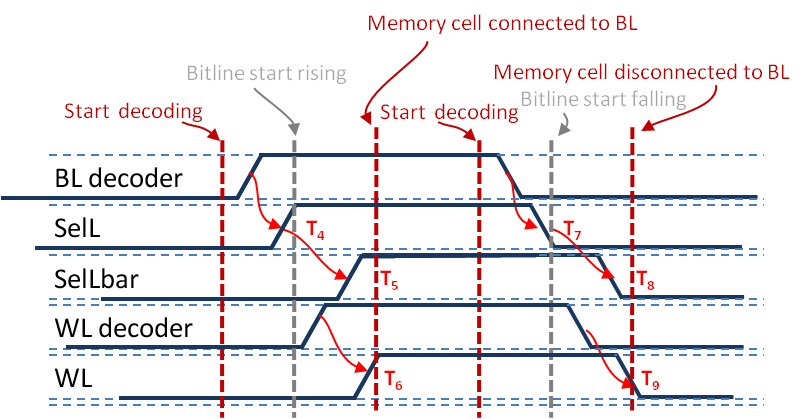
\includegraphics[scale=0.9]{../fig/hfdstk-timing-lbcell2.png}
  \caption[Data-array:timing]{Timing controlelogica data-array}
  \label{fig:lbcell_timing2}
\end{figure}

\begin{figure}[!ht]
  \centering
  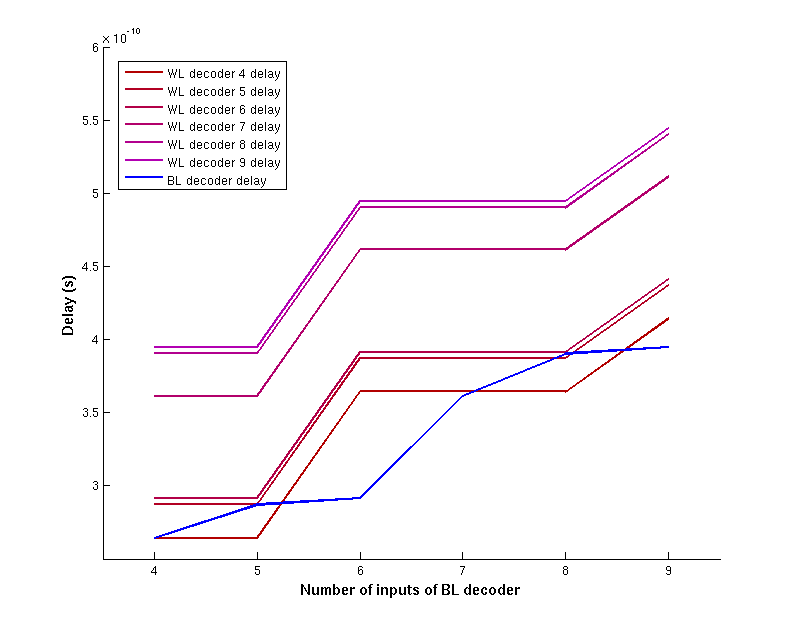
\includegraphics[scale=0.6]{../fig/hfdstk-timing-decoder-dep.png}
  \caption[Delay van WL-decoders en -buffers i.f.v. BL-decoders]{Delay van WL-decoders en -buffers i.f.v. aantal bitlijnen}
  \label{fig:decoder_dep}
\end{figure}

\paragraph{}
De timingvoorwaarden voor het selecteren en deselecteren van de referentiecellen zijn dezelfde als die van de datacellen. Het circuit- en timingdiagramma hiervan zijn geïllustreerd in figuren \ref{fig:lbref_timing1} en \ref{fig:lbref_timing2}. Anders als bij de datacellen is er aan de timingvoorwaarden al automatisch voldaan met deze logica. Dit omdat de WLs worden aangestuurd door een signaal dat rechtstreeks van de BL-decoder komt. Dit signaal word dan vertraagd met twee invertoren om de juiste timing te verwezenlijken.


\begin{figure}[!ht]
  \centering
  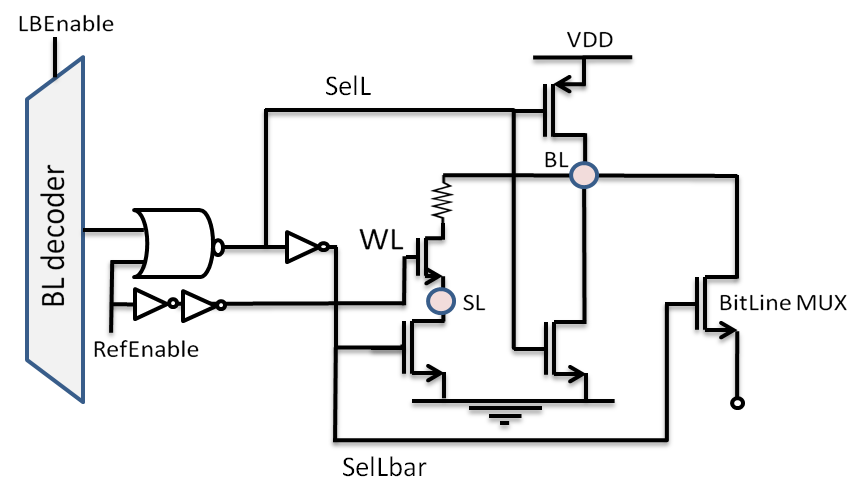
\includegraphics[scale=0.6]{../fig/hfdstk-timing-lbref1.png}
  \caption[Referentie-array:logica]{Controlelogica referentie-array}
  \label{fig:lbref_timing1}
\end{figure}

\begin{figure}[!ht]
  \centering
  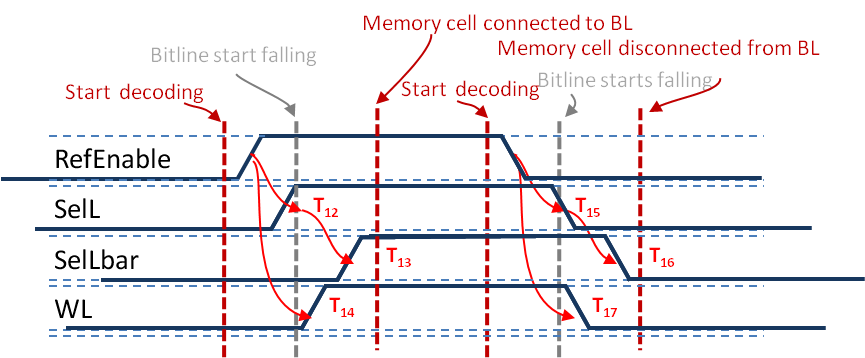
\includegraphics[scale=0.9]{../fig/hfdstk-timing-lbref2.png}
  \caption[Referentie-array:timing]{Timing controlelogica referentie-array}
  \label{fig:lbref_timing2}
\end{figure}

\subsection{Kritische timing voor het uitlezen van de cel}
Eens de cel geselecteerd is wordt de bitline opgeladen. De volgende stap is dit signaal te voeden aan de sense amplifier. Het signaal wordt eerst door een eerste passgate geleid om uit het local block te geraken. Vervolgens wordt het signaal door een tweede passgate geleid die als sample-and-hold dient voor de sense amplifier. Figuren \ref{fig:sa_timing1} en \ref{fig:sa_timing2} illustreren het circuit en timing rond de sense amplifier. Eens de BL wordt aangesproken wordt de eerste passgate automatisch geactiveerd zoals uitgelegd in de vorige paragrafen. T19 stelt het tijdstip voor wanneer de tweede passgate aangezet moet worden. Deze timing is niet cruciaal: de tweede passgate mag zowel voor als na de eerste passgate geactiveerd worden. Het tijdstip waarop deze passgate wordt afgeschakeld (T22) is daarentegen wel belangrijk. Dit moet namelijk gebeuren voordat de eerste passgate afgesloten is (T21), indien niet zullen er 2 ladingsinjectie optreden i.p.v. één. Om een zo snel mogelijke latching van de sense amplifier te verkrijgen, is het tijdstip waarop de sense amplifier (T20) geactiveerd wordt belangrijk. Wanneer de sense amplifier juist wordt aangesloten treedt er het RC-latch-effect op waarbij de SA zich gedraagt alsof er geen last aan hangt. Dit effect werd beschreven in sectie \ref{RC-latch-effect}. Na deze snelle fase, gaan de ingangs-uitgangsknopen van de SA veel trager opladen en gaat de SA de BL ook op- of ontladen. Om een snelle latching te verkrijgen moet de tweede passgate dus zo snel mogelijk na de snelle fase afgeschakeld worden. Eens de ingangs-uitgangsknopen van de SA gelatcht zijn, mag de SA gedesactiveerd worden.

\begin{figure}[!ht]
  \centering
  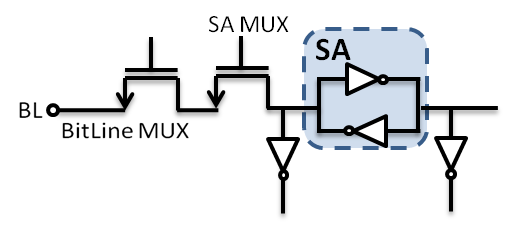
\includegraphics[scale=0.6]{../fig/hfdstk-timing-sa1.png}
  \caption[SA:logica]{Logica rond SA}
  \label{fig:sa_timing1}
\end{figure}

\begin{figure}[!ht]
  \centering
  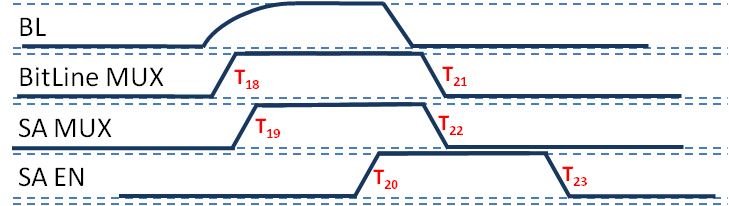
\includegraphics[scale=0.9]{../fig/hfdstk-timing-sa2.png}
  \caption[SA:timing]{Timing logica rond SA}
  \label{fig:sa_timing2}
\end{figure}

\section{Analyse verschillende geheugenconfiguraties}
\paragraph{}
Het finale geheugen is 1Mbit groot. Heel wat configuraties zijn mogelijk om dit te verwezenlijken. Om deze mogelijkheden wat in te perken wordt volgende beperking opgelegd: het aantal WLs moet groter dan of gelijk zijn aan het aantal BLs. Bij deze configuraties zal het ontladen van de bitlijn sneller verlopen dan bij configuraties met meer BLs dan WLs. Dit levert 20 mogelijke configuraties voor NoWLpB, NoBLpLB en NoGB. Deze configuraties worden vergeleken op basis van oppervlakte, energieverbruik en leessnelheid. 

\subsection{Evaluatie criteria voor de geheugenconfiguraties}
De oppervlakte wordt berekend op basis van de lengtes en breedtes van het totaal aantal transistoren (behalve de celtransistoren). Verbindingslijnen worden niet meegerekend in de berekeningen van de oppervlakte van de logica. Voor de lengte van de geheugencellen wordt 1.5*6F genomen en voor de breedte wordt 2*6F genomen \cite{ppt:cosemans}. Hoewel deze afmetingen voor een MTJ geheugen cell zijn, geven ze een goede schatting van de oppervlakte van een 1T1R-cel. Deze oppervlakte omvat ook de oppervlakte van bitlijn, woordlijn en sourcelijn meegerekend. \\
Het energie verbruik wordt berekend door de stroom van de voedingsspanning te integreren over de tijd en te vermenigvuldigen met de voedingsspanning. De signalen die binnen komen in een global block zijn in SPICE simulaties afkomstig van ideale spanningsbronnen. Dit heeft als gevolg dat er een ladingsinjectie optreedt naar de voedingsspanningsbron (zie bijlage \ref{app:chargeinj}). Dit heeft een beperkte invloed op de energieberekeningen. Deze invloed wordt evenwel niet meegenomen in de analyse. \\
De leessnelheid is afhankelijk van de verschillende controlesignalen in de leescyclus. De simulatie-opstelling is als volgt: de leescyclus begint wanneer de signalen binnen komen in het global block. De SA wordt aangezet wanneer het verschil tussen de data- en referentiesignaal 100mV bedraagt. Omdat er niet gewacht wordt op het tijdstip wanneer de BL volledig opgeladen is, wordt het verschil in leessnelheid tussen geheugens met een klein aantal woordlijnen en geheugens met een groot aantal woordlijnen vergroot. Geheugens met iets meer woordlijnen worden zo in de race gehouden. In het finale geheugenontwerp zal de leessnelheid verder opgedreven worden door dit 100mV spanningsverschil te verkleinen. Verder wordt er ook altijd een HRS-cel uitgelezen aangezien deze de bitlijn langer moet opladen om tot aan de 100mV verschildrempel te komen wat een realistischere leessnelheid geeft. De leescyclus eindigt wanneer de BL-spanning terug naar de grond is getrokken. Figure \ref{fig:leescyclus} illustreert de hele leescyclus.

\begin{figure}[!ht]
  \centering
  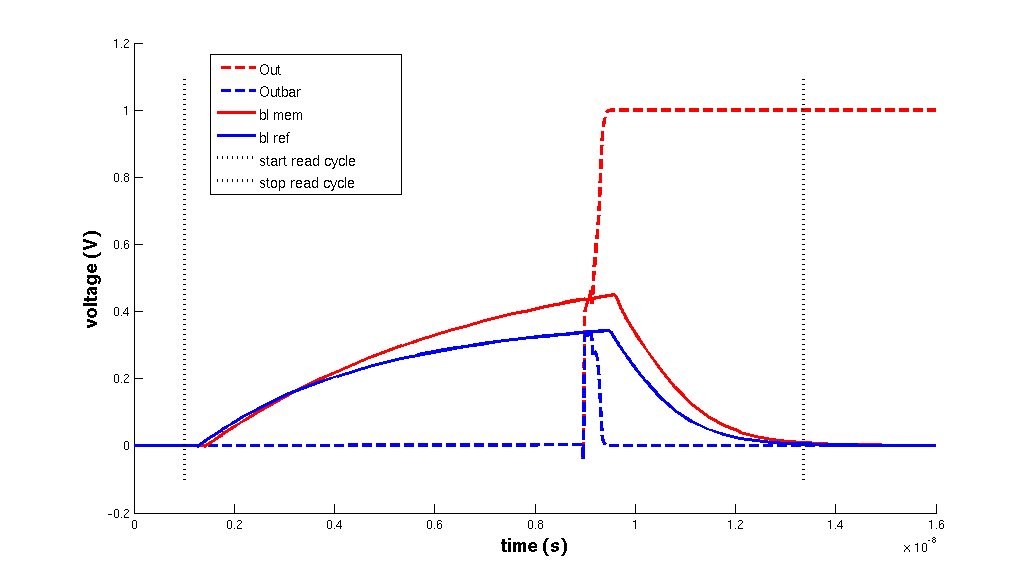
\includegraphics[width=0.9\textwidth]{../fig/hfdstk-timing-leescyclus.png}
  \caption[Leescyclus]{Leescyclus}
  \label{fig:leescyclus}
\end{figure} 

\subsection{Vergelijking van de geheugenconfiguraties}
Er werden 20 mogelijke geheugenconfiguraties geselecteerd als kandidaat voor het finale ontwerp, hun positie in de evaluatieruimte wordt getoond in figuur \ref{fig:final20all1}. Hierop staat het energieverbruik op de x-as, delay op de y-as en de oppervlakte wordt weergegeven door de grootte van de bolletjes. Het aantal effectief gebruikte referentiecellen wordt constant gehouden voor de verschillende configuraties. Dit wordt gedaan om het energieverbruik te verkleinen en omdat men maar een beperkt aantal cellen nodig heeft om een goede referentiedistributie te verkrijgen. De delay wordt voornamelijk bepaald door het opladen van de bitlijnen, die ook de grootste energieverbruikers zijn. De snelheid van de bitlijnen wordt dan weer bepaald door het aantal woordlijnen, dit kan gezien worden in figuur \ref{fig:final20all2}. Het aantal bitlijnen beinvloedt dan weer meer het energieverbruik. Dit extra energieverbruik gaat in de eerste plaats naar de WL-buffers, in mindere mate naar de bitlijn decoders en nog minder naar de bitlijn zelf. Bij alle geheugenconfiguraties komt het vermogenverbruik voornamelijk van de geheugecel, vervolgens in dalende lijn van de logica, de buffers en de sense amplifiers. De oppervlakte wordt bepaald door het aantal global blocks en de grootte van de decoders. Een groot aantal woordlijnen in combinatie met een klein aantal bitlijnen geeft de noodzaak aan een groot aantal global blocks, dit heeft een groot oppervlak als gevolg.\\
Er kan dus besloten worden dat een geheugen configuratie bestaande uit een klein aantal woordlijnen en evenveel bitlijnen een optimum zal geven voor energieverbruik en delay, maar een suboptimum voor oppervlakte.

\afterpage{
\begin{figure}[!ht]
  \centering
  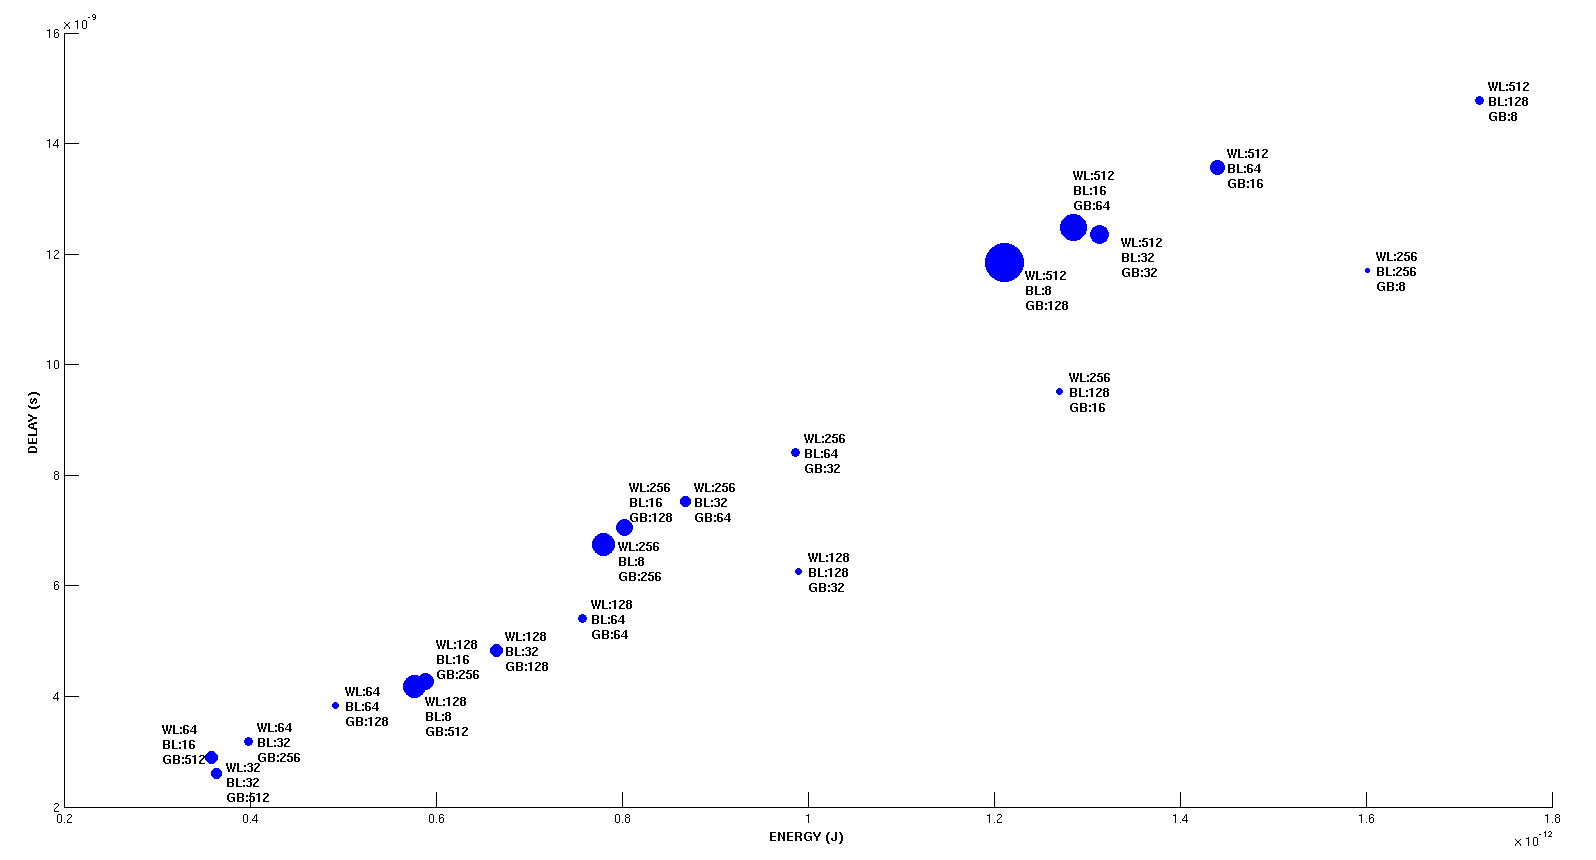
\includegraphics[scale=0.45, angle = 90]{../fig/hfdstk-timing-all-sol1.png}
  \caption[Delay, energieverbruik en oppervlakte van alle geheugenconfiguraties]{Delay, energieverbruik en oppervlakte van verschillende geheugenconfiguraties van 1Mbit. Kleinste transistor-gate-oppervlakte is $0.009mm^{2}$, grootste transistor-gate-oppervlakte is $0.68mm^{2}$}
  \label{fig:final20all1}
\end{figure} 
\clearpage
}

\begin{figure}[!ht]
  \centering
  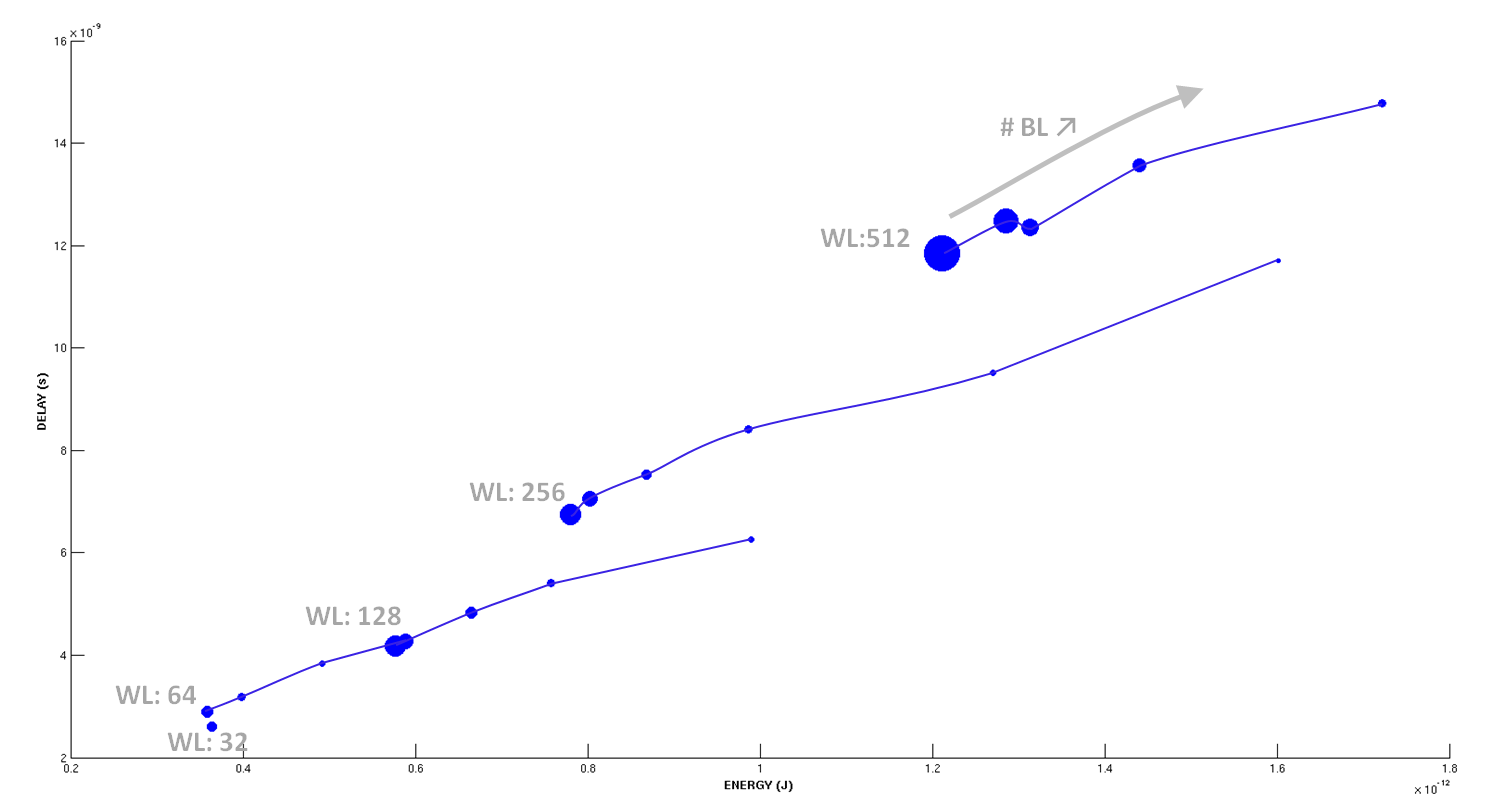
\includegraphics[scale=0.6]{../fig/hfdstk-timing-all-sol2.png}
  \caption[Delay, energieverbruik en oppervlakte van alle geheugenconfiguraties]{Invloed \#BL en \#WL op delay, energieverbruik en oppervlakte voor verschillende geheugenconfiguraties van 1Mbit. Kleinste transistor-gate-oppervlakte is $0.009mm^{2}$, grootste transistor-gate-oppervlakte is $0.68mm^{2}$}
  \label{fig:final20all2}
\end{figure} 

\section{Besluit}
In dit hoofdstuk werd de timing van alle logica in de geheugenarchitectuur in kaart gebracht. Hierbij werd er gekeken naar wat de gewenste opeenvolging van signalen is en hoe dit problemen of beperkingen in de architectuur kan teweegbrengen. Vervolgens werd met deze kennis een aantal geheugenconfiguraties ontworpen en vergeleken. De conclusie is dat een kleiner aantal woordlijnen en bitlijnen een optimale snelheid en energieverbruik voor een GB geven. Op het vlak van oppervlakte leidt dit tot een suboptimum.
